\documentclass[11pt, a4paper]{article}

% ── Lengua ─────────────────────────────
\usepackage[utf8]{inputenc}
\usepackage[T1]{fontenc}
\usepackage[spanish]{babel}

% ── Fuentes compatibles pdflatex ───────
\usepackage{lmodern}
\usepackage{courier}

% ── Interlineado ───────────────────────
\usepackage{setspace}
\onehalfspacing

% ── Márgenes ───────────────────────────
\usepackage[a4paper, margin=2.5cm]{geometry}

% ── Cabecera/pie ───────────────────────
\usepackage{fancyhdr}
\pagestyle{fancy}
\fancyhf{}
\rfoot{\thepage}
\renewcommand{\headrulewidth}{0pt}

% ── Imágenes ───────────────────────────
\usepackage{graphicx}
\graphicspath{{imgs/}}
\usepackage{subcaption}

% ── Links ──────────────────────────────
\usepackage[hidelinks]{hyperref}

% ── Código ─────────────────────────────
\usepackage{listings}
\lstset{
  basicstyle=\ttfamily\footnotesize,
  breaklines=true,
  frame=single,
  numbers=left,
  numberstyle=\tiny
}

% ── Math ────────────────────────────────
\usepackage{amsmath}
\usepackage{float}

\usepackage{booktabs}

% ── Documento ───────────────────────────
\begin{document}

% ── PORTADA ─────────────────────────────
\begin{titlepage}
\centering

% empuja todo hacia el centro vertical
\vspace*{\fill}

{\Huge \textbf{Actividad 3, Estadística inferencial: del análisis muestral a 
la predicción poblacional}\par}

\vspace{1.5cm}

{\Large David Vicente Moya\par}

\vspace{0.5cm}

{\large \today\par}

% relleno inferior para centrar verticalmente
\vspace*{\fill}

\end{titlepage}

% ── ÍNDICE ──────────────────────────────
\newpage
\tableofcontents
\thispagestyle{empty}
\setcounter{page}{0}

% ── CONTENIDO ──────────────────────────
\newpage

\section{¿Qué son y para qué se utilizan los contrastes de hipótesis?}

En la vida diaria tomamos decisiones constantemente a partir de información incompleta: si 
un nuevo método de paquetería es realmente más rápido que el anterior, si un medicamento 
funciona mejor que un placebo, o si dos grupos de clientes gastan de forma distinta. Casi 
nunca disponemos de los datos de toda la población sino solo de una muestra. Un 
\textbf{contraste de hipótesis} es la herramienta estadística que permite responder a este 
tipo de preguntas de forma rigurosa: nos dice si la diferencia que observamos en una 
muestra es lo bastante grande como para concluir que existe realmente en la población, o si 
por el contrario, puede explicarse simplemente por el azar propio del muestreo.

La lógica del contraste parte siempre de dos afirmaciones contrapuestas sobre la población. 
La primera, llamada \textbf{hipótesis nula} ($H_0$), representa la situación de partida: 
"no hay diferencia", "el efecto no existe", "todo sigue igual que antes". La segunda, 
la \textbf{hipótesis alternativa} ($H_1$), es lo que nos interesa demostrar: "sí hay una 
diferencia", "el nuevo método mejora el tiempo de entrega", "los dos grupos no se comportan 
igual". El contraste de hipótesis no demuestra cuál de las dos es verdadera de forma 
absoluta, en su lugar evalúa si la evidencia de la muestra es suficientemente fuerte como 
para \textbf{rechazar} la hipótesis nula a favor de la alternativa.

Estos contrastes se utilizan en prácticamente cualquier disciplina que trabaje con datos: 
en medicina, para comprobar si un tratamiento es eficaz; en ingeniería, para verificar si 
un proceso productivo cumple un estándar de calidad; en marketing y negocio, para decidir 
si una campaña ha aumentado las ventas. En definitiva, los contrastes de hipótesis 
convierten el (\textit{"creo que esto ha cambiado"}) en una 
conclusión respaldada por datos, con un nivel de confianza cuantificado.

\section{Algoritmo general para realizar un contraste de hipótesis}

\subsection{Caso de una población}

Para contrastar una hipótesis sobre el parámetro de una única población (habitualmente la 
media $\mu$), se sigue el siguiente procedimiento general:

\begin{enumerate}
  \item \textbf{Formular las hipótesis.} Se establece la hipótesis nula $H_0: \mu = \mu_0$ 
  y la hipótesis alternativa $H_1$, que puede ser bilateral ($\mu \neq \mu_0$) o unilateral 
  ($\mu > \mu_0$ o $\mu < \mu_0$), según lo que se desee investigar.

  \item \textbf{Fijar el nivel de significación} $\alpha$ (habitualmente 0.05), que 
  representa la probabilidad máxima admitida de rechazar $H_0$ siendo realmente cierta 
  (error de tipo I).

  \item \textbf{Elegir el estadístico de contraste}, según si se conoce o no la varianza 
  poblacional $\sigma^2$:
  \begin{itemize}
    \item Si $\sigma^2$ es \textbf{conocida} (o el tamaño muestral es grande, $n \geq 30$, 
    apoyándonos en el Teorema Central del Límite), se utiliza el estadístico $Z$:
    \[
    Z = \frac{\bar{x} - \mu_0}{\sigma / \sqrt{n}}
    \]
    que sigue una distribución normal estándar $N(0,1)$ bajo $H_0$.

    \item Si $\sigma^2$ es \textbf{desconocida} (caso habitual en la práctica) y se estima 
    a partir de la cuasivarianza muestral $s$, se utiliza el estadístico $t$ de Student:
    \[
    t = \frac{\bar{x} - \mu_0}{s / \sqrt{n}}
    \]
    que sigue una distribución $t$ de Student con $n-1$ grados de libertad.
  \end{itemize}

  \item \textbf{Calcular el valor del estadístico} a partir de los datos de la muestra 
  ($\bar{x}$, $s$, $n$).

  \item \textbf{Obtener el p-valor} 
  \begin{itemize}
    \item Si $P < \alpha$: Rechaza $H_0$. Las diferencias son estadísticamente significativas.
    \item Si $P \geq \alpha$: No rechaza $H_0$. No hay evidencia suficiente para descartarla.
  \end{itemize}

  \item \textbf{Interpretación:} Se forman conclusiones y se discuten los hallazgos del análisis.
\end{enumerate}

\subsection{Caso de comparación de dos poblaciones}

Cuando el objetivo es comparar el mismo parámetro entre dos poblaciones independientes se emplea 
un procedimiento casi idéntico, pero el estadístico se construye sobre la diferencia de 
medias:

\begin{enumerate}
  \item \textbf{Formular las hipótesis:} $H_0: \mu_1 = \mu_2$ frente a $H_1: \mu_1 \neq \mu_2$ (o unilateral, $\mu_1 > \mu_2$).

  \item \textbf{Fijar el nivel de significación} $\alpha$.

  \item \textbf{Elegir el estadístico}, de nuevo según el conocimiento de las varianzas 
  poblacionales:
  \begin{itemize}
    \item Con varianzas desconocidas (caso habitual), estadístico $t$ de Student para dos muestras independientes:
    \[
    t = \frac{(\bar{x}_1 - \bar{x}_2) - (\mu_1 - \mu_2)}{\hat{S}\sqrt{\dfrac{1}{n_1} + \dfrac{1}{n_2}}}
    \]
  \end{itemize}

  \item \textbf{Calcular el estadístico} con las medias, varianzas y tamaños muestrales de ambos grupos.

  \item \textbf{Obtener el p-valor} asociado al estadístico bajo la distribución correspondiente.

  \item \textbf{Interpretar} los resultados obtenidos.
\end{enumerate}


\section{Planteamiento de los escenarios}

Para esta actividad he utilizado el conjunto de datos 
\textit{E-Commerce Customer Behavior \& Sales Analysis}, disponible públicamente en Kaggle 
(\url{https://www.kaggle.com/datasets/umuttuygurr/e-commerce-customer-behavior-and-sales-analysis-tr}), 
con 5000 registros de pedidos individuales. En esta sección se proponen dos escenarios 
hipotéticos en el que asumo el cargo de analista de datos dentro de una empresa de comercio
digital.

\subsection{Escenario A: contraste sobre una población (tiempo de entrega)}

Una empresa de comercio digital promete a sus clientes un tiempo de entrega medio de 5 
días desde la confirmación del pedido. El departamento de operaciones quiere comprobar, a 
partir de los pedidos registrados, si en la práctica el tiempo de entrega real supera al 
comprometido.

\textbf{Variable analizada:} \texttt{Delivery\_Time\_Days}, el número de días transcurridos 
entre la realización del pedido y su entrega, registrado para cada pedido individual.

\textbf{Hipótesis:}
\[
H_0: \mu = 5 \qquad \text{frente a} \qquad H_1: \mu > 5
\]

Se trata de un contraste unilateral: no interesa solo si el tiempo medio de entrega es 
distinto de 5 días, sino específicamente si lo \textbf{supera}, ya que esa es la situación 
que afecta negativamente a la satisfacción del cliente.

\subsection{Escenario B: contraste entre dos poblaciones (gasto de clientes nuevos y recurrentes)}

El equipo de marketing quiere saber si los clientes que ya han comprado anteriormente 
(clientes recurrentes) gastan, por lo general, más por pedido que los clientes que compran 
por primera vez. Esta información es relevante para decidir si merece la pena invertir en 
estrategias de fidelización.

\textbf{Variable analizada:} \texttt{Total\_Amount}, el importe total gastado en cada pedido, 
comparado entre dos grupos independientes definidos por la variable 
\texttt{Is\_Returning\_Customer} (cliente recurrente vs. cliente nuevo).

\textbf{Hipótesis:}
\[
H_0: \mu_{\text{recurrente}} = \mu_{\text{nuevo}} \qquad \text{frente a} \qquad H_1: \mu_{\text{recurrente}} > \mu_{\text{nuevo}}
\]

Se trata también de un contraste unilateral, puesto que la hipótesis de interés del negocio 
es específicamente que los clientes recurrentes gastan \textbf{más}, no que ambos grupos 
sean diferentes.

\section{Modelos numéricos}

\subsection{Escenario A: tiempo de entrega}

\subsubsection{Estadística descriptiva}

A partir de los 5000 pedidos registrados en la base de datos, el tiempo de entrega presenta 
los siguientes estadísticos descriptivos:

\begin{center}
\begin{tabular}{lc}
\toprule
Estadístico & Valor (días) \\
\midrule
Mínimo & 1.000 \\
1er cuartil & 4.000 \\
Mediana & 6.000 \\
Media & 6.497 \\
3er cuartil & 8.000 \\
Máximo & 25.000 \\
Desviación típica & 3.465 \\
\bottomrule
\end{tabular}
\end{center}

La Figura~\ref{fig:hist_delivery} muestra la distribución del tiempo de entrega. Se observa 
una distribución asimétrica a la derecha, con la mayor concentración de pedidos entre 2 y 8 
días, y una cola larga de pedidos con tiempos de entrega excepcionalmente altos (hasta 25 
días). La línea discontinua roja marca la media muestral (6.497 días), claramente por 
encima de los 5 días que la empresa promete a sus clientes.

\begin{figure}[H]
  \centering
  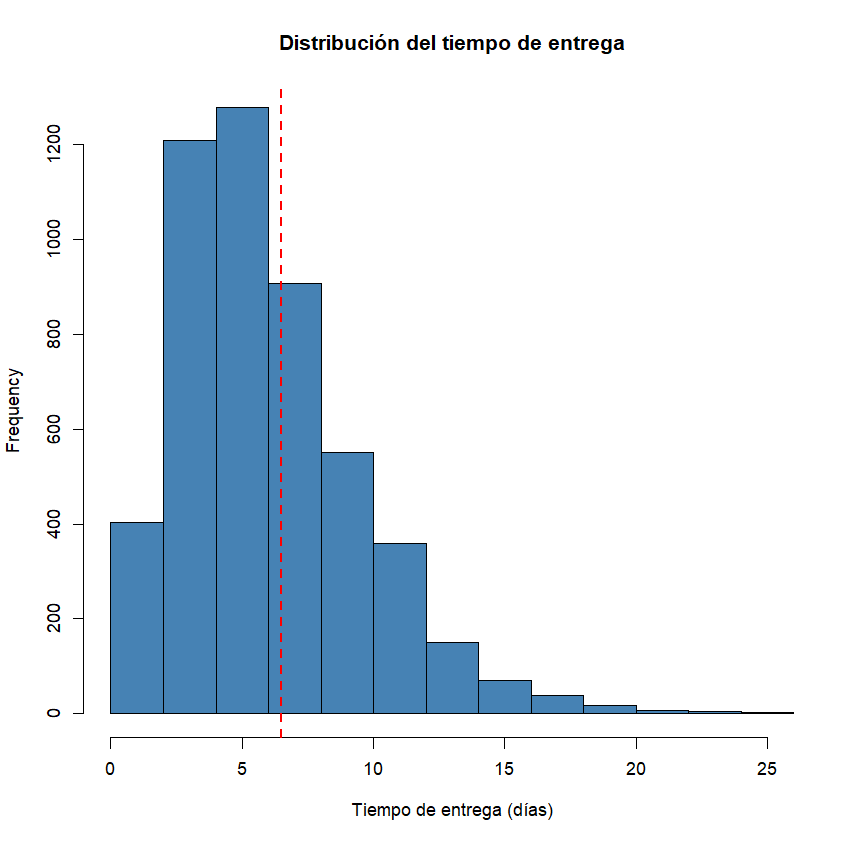
\includegraphics[width=0.7\textwidth]{frecuencia_tiempo_entrega.png}
  \caption{Distribución del tiempo de entrega de los pedidos.}
  \label{fig:hist_delivery}
\end{figure}

\subsubsection{Contraste de hipótesis}

Se aplica un contraste t de una muestra, dado que la varianza poblacional es desconocida y 
se estima a partir de los datos:

\[
H_0: \mu = 5 \qquad \text{frente a} \qquad H_1: \mu > 5
\]

Los resultados obtenidos en son:

\begin{center}
\begin{tabular}{lc}
\toprule
Estadístico & Valor \\
\midrule
$t$ & 30.55 \\
Grados de libertad & 4999 \\
p-valor & $< 2.2 \times 10^{-16}$ \\
IC 95\% (inferior) & 6.416 \\
Media muestral & 6.497 \\
\bottomrule
\end{tabular}
\end{center}

Dado que el p-valor ($< 2.2 \times 10^{-16}$) es muchísimo menor que $\alpha = 0.05$, se 
\textbf{rechaza $H_0$}. Existe evidencia estadística muy fuerte de que el tiempo medio de 
entrega real es superior a los 5 días prometidos por la empresa.

\subsection{Escenario B: gasto de clientes nuevos y recurrentes}

\subsubsection{Estadística descriptiva}

La base de datos contiene 2010 pedidos de clientes nuevos y 2990 pedidos de clientes 
recurrentes. La Tabla~\ref{tab:desc_gasto} resume los estadísticos descriptivos del importe 
total del pedido (\texttt{Total\_Amount}) para cada grupo.

\begin{table}[H]
\centering
\begin{tabular}{lcc}
\toprule
Estadístico & Cliente nuevo & Cliente recurrente \\
\midrule
n & 2010 & 2990 \\
Mínimo & 7.87 & 7.89 \\
1er cuartil & 120.03 & 125.78 \\
Mediana & 326.71 & 348.71 \\
Media & 978.87 & 985.96 \\
3er cuartil & 939.50 & 1002.66 \\
Máximo & 22023.90 & 21478.35 \\
Desviación típica & 2005.09 & 1824.52 \\
\bottomrule
\end{tabular}
\caption{Estadística descriptiva del gasto por tipo de cliente.}
\label{tab:desc_gasto}
\end{table}

Ambos grupos presentan medias muy similares (978.87 frente a 985.96) y una fuerte asimetría 
a la derecha, con medianas muy por debajo de la media y máximos que superan los 20000, lo 
que indica la presencia de pedidos puntuales de muy alto valor.

La Figura~\ref{fig:boxplot_gasto} muestra un diagrama de cajas comparativo, representado en 
escala logarítmica en el eje vertical debido a la fuerte asimetría de la variable. Se 
observa que ambas distribuciones son prácticamente idénticas en mediana, rango 
intercuartílico y presencia de valores atípicos, lo que sugiere que no existe una 
diferencia relevante de gasto entre ambos grupos de clientes.

\begin{figure}[H]
  \centering
  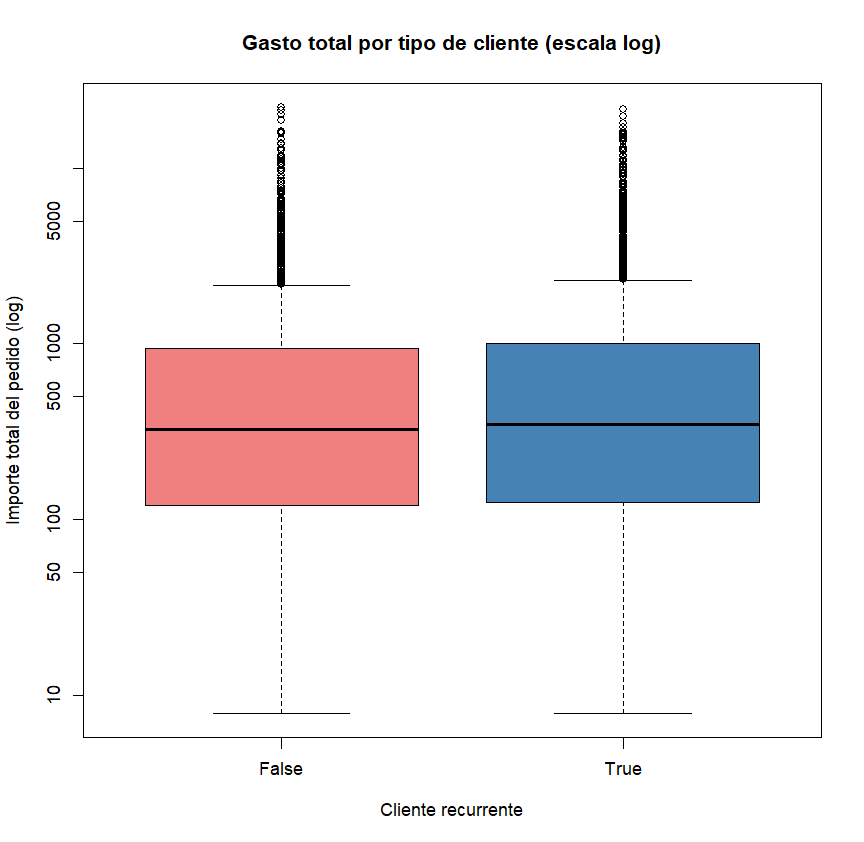
\includegraphics[width=0.7\textwidth]{gasto_tipo_cliente.png}
  \caption{Diagrama de cajas del gasto total por tipo de cliente (escala logarítmica).}
  \label{fig:boxplot_gasto}
\end{figure}

\subsubsection{Contraste de hipótesis}

Dado que las varianzas de ambos grupos son desconocidas y no se puede asumir que sean 
iguales, se aplica el test t para dos muestras independientes:

\[
H_0: \mu_{\text{recurrente}} = \mu_{\text{nuevo}} \qquad \text{frente a} \qquad H_1: \mu_{\text{recurrente}} > \mu_{\text{nuevo}}
\]

Los resultados obtenidos en son:

\begin{table}[H]
\centering
\begin{tabular}{lc}
\toprule
Estadístico & Valor \\
\midrule
$t$ & $-0.127$ \\
Grados de libertad  & 4028.9 \\
p-valor & 0.4494 \\
IC 95\% (superior) & 84.71 \\
Media (cliente nuevo) & 978.87 \\
Media (cliente recurrente) & 985.96 \\
\bottomrule
\end{tabular}
\caption{Resultados del contraste de hipótesis para el Escenario B.}
\label{tab:test_gasto}
\end{table}

Dado que el p-valor (0.4494) es muy superior a $\alpha = 0.05$, \textbf{no se rechaza $H_0$}. 
No existe evidencia estadística suficiente para afirmar que los clientes recurrentes gastan 
más por pedido que los clientes nuevos. La pequeña diferencia observada en las medias 
muestrales es atribuible al azar del muestreo.

\section{Conclusiones}

Los dos escenarios analizados han arrojado resultados opuestos, lo cual resulta 
útil desde un punto de vista didáctico: no todo contraste de hipótesis termina en el 
rechazo de $H_0$, y un resultado "no significativo" es tan informativo como uno que sí lo es.

En el \textbf{Escenario A}, el contraste mostró que el tiempo medio real de entrega 
(6.497 días) es significativamente superior al compromiso de 5 días asumido para la empresa 
($p < 2.2 \times 10^{-16}$). Esto representa una señal de alerta: si una empresa real 
promete un plazo de entrega y sistemáticamente lo incumple, puede generar insatisfacción y 
pérdida de confianza en los clientes, independientemente de que el incumplimiento medio 
(1.5 días aproximadamente) no parezca muy elevado.

En el \textbf{Escenario B}, en cambio, no se encontró evidencia de que los clientes 
recurrentes gasten más por pedido que los clientes nuevos ($p = 0.4494$). La diferencia 
observada entre las medias (978.87 frente a 985.96) es mínima y queda dentro del rango que 
se podría esperar por el azar del muestreo. Esto implica que no estaría justificado diseñar 
estrategias de fidelización basadas en la expectativa de que un cliente recurrente vaya a 
gastar más por compra. Si existiese valor en la fidelización, habría que buscarlo en otra 
variable, como la frecuencia de compra o el valor acumulado a lo largo del tiempo, en lugar 
del importe de cada pedido individual.

Resulta interesante comparar por qué un caso resultó significativo y el otro no. En el 
Escenario A, la diferencia entre la media observada y el valor de referencia 
($6.497 - 5 = 1.497$) era grande en relación con la variabilidad de los datos 
(desviación típica de 3.46, pero con un tamaño muestral de 5000 que reduce mucho el error). 
En el Escenario B, la diferencia entre los dos grupos es minúscula frente a una 
desviación típica de entre 1800 y 2000.

Por último, conviene señalar dos limitaciones del análisis. En primer lugar, ambos 
escenarios se han construido sobre la misma base de datos, por lo que no constituyen 
evidencias independientes sobre el comportamiento general del comercio electrónico, sino 
observaciones específicas de esta empresa concreta. En segundo lugar, el valor de 
referencia utilizado en el Escenario A ($\mu_0 = 5$ días) es un supuesto razonado sobre un 
compromiso de entrega típico del sector, y no un dato contractual verificado de la empresa, 
por lo que la conclusión debe interpretarse en ese contexto.

\end{document}